\documentclass[11pt]{article}
\usepackage[margin=1in]{geometry}
\usepackage[T1]{fontenc}
\usepackage[utf8]{inputenc}
\usepackage{lmodern}
\usepackage{amsmath}
\usepackage{booktabs}
\usepackage{graphicx}
\usepackage{caption}
\usepackage{float}
\usepackage[hidelinks]{hyperref}
\captionsetup{font=small,labelfont=bf}
\graphicspath{{figures/}}
\newcommand{\GST}{Ge$_2$Sb$_2$Te$_5$}
\newcommand{\nozbl}{\texttt{nequip\_no\_zbl}}

\title{Melt-quench of \GST{} with 0--10 at.\% carbon\\ with the no-ZBL Allegro potential \nozbl}
\author{\texttt{cgst\_allegro\_sims}, \texttt{meltquench/results/nequip\_no\_zbl}}
\date{November 2026}

\begin{document}
\maketitle

\begin{abstract}
Amorphous \GST{} with 0, 1.07, 2.54, 5.14 and 9.96 at.\% C was made by melt-quench molecular dynamics with the
Allegro potential \nozbl{}, which has no short-range (ZBL) repulsion, in $4\times4\times4$ cells of 29.5k--32.8k
atoms: three replicas per composition at 10\,K/ps, and one at 5 and one at 1\,K/ps for 0 and 10\% C. No atom pair
came closer than 1.08\,\AA{} in any liquid, so the missing ZBL term did not show. Carbon lowers the density (by
2.3\% in the glass at 10\% C) and the apparent melting point (1139 to 978\,K), and it segregates, with 87\% of C atoms
bonded to other C at 10\% C. The 0\% C glass is as dense as the model's crystal and as dense as the DFT reference's
own glass. A 1\,K/ps quench partly crystallizes the glass (crystal-like Ge/Sb/Te fraction 0.30 at 0\% C and 0.21 at
10\% C, against 0.14 and 0.13 at 10\,K/ps), while 5\,K/ps changes the glass only slightly; the recrystallization
study therefore starts from the 10\,K/ps glasses. The same protocol will be run with the two potentials that add a
ZBL term (\texttt{nequip\_zbl}, \texttt{rushik\_zbl\_pairwise}); this report covers \nozbl{} alone.
\end{abstract}

\section{Method}
The starting structures are $4\times4\times4$ rocksalt supercells of \GST{} with C on cation-vacancy sites; the 10\%
C cell has every vacancy filled, so it differs from the others in vacancy count as well as C content. All runs are
NPT at 0\,bar (isotropic Nos\'e--Hoover, $T_\text{damp}=100\,\Delta t$, $P_\text{damp}=1000\,\Delta t$,
$\Delta t=2$\,fs, checked for energy conservation with this potential), on two A100 GPUs per run (three A30s for the
5\,K/ps runs):

\begin{table}[H]
\centering
\begin{tabular}{lll}
\toprule
Stage & Temperature & Duration \\
\midrule
Minimize and equilibrate the crystal & 300\,K & 20\,ps \\
Heat & 300 $\to$ 1500\,K & 120\,ps (10\,K/ps) \\
Melt; MSD gate: every species $\geq 100$\,\AA$^2$ & 1500\,K & 100\,ps \\
Quench & 1500 $\to$ 300\,K & 120, 240 or 1200\,ps (10, 5 or 1\,K/ps) \\
Glass: relax, then average & 300\,K & 50 + 50\,ps \\
\bottomrule
\end{tabular}
\end{table}

The melt temperature and hold were confirmed by a pilot (0 and 10\% C): 1500\,K is 361\,K above the highest apparent
melting point, and the smallest per-species mean squared displacement in the hold was 349--651\,\AA$^2$ over all runs,
against a gate of 100\,\AA$^2$. Coordination uses fixed bond cutoffs (3.2\,\AA{} between Ge/Sb/Te, 2.5\,\AA{} for
C--Ge/Sb/Te, 1.9\,\AA{} for C--C; Section~\ref{sec:cutoffs}). Crystal-like order is \texttt{xfracGST}, the fraction of
Ge/Sb/Te atoms with at least four crystal-like Steinhardt-$q_4$ bonds (default criterion 3.6\,\AA, 0.5, 4; the calibrated recrystallization criterion is a separate study).

\section{Close contacts without ZBL}
Without a short-range repulsive term, nothing but the training data keeps atoms apart at very short range, and the
risk is greatest in the hot liquid. The closest approach of each pair type was read from the radial distribution
functions of the 1500\,K liquid (last 20\,ps of the hold) and the 300\,K glass:

\begin{table}[H]
\centering
\caption{Closest approach (\AA), liquid at 1500\,K / glass at 300\,K, range over all 10\,K/ps runs that contain the pair.}
\begin{tabular}{ll}
\toprule
Pairs & \nozbl{} \\
\midrule
Ge/Sb/Te pairs & $\geq 1.98$ / $\geq 2.24$ \\
Ge--C & 1.62--1.64 / 1.78--1.84 \\
Te--C & 1.72--1.80 / 1.88--1.98 \\
C--C & 1.08--1.12 / 1.16--1.20 \\
\bottomrule
\end{tabular}
\end{table}

No pair came below 1.0\,\AA, and the C--C minimum sits just below the short end of real C--C bonds (1.2--1.5\,\AA)
in the liquid and at it in the glass. The 2\,fs timestep conserves energy in the 1500\,K 10\%
C liquid (drift $\leq 0.0002$\,meV/atom/ps). For this protocol the missing ZBL term caused no
close contacts; whether a ZBL term changes the closest approaches is the first comparison to make with the other two
potentials.

\section{Thermodynamic properties}

\begin{table}[H]
\centering
\caption{Properties against C content, 10\,K/ps, mean $\pm$ sample standard deviation over three replicas.}
\footnotesize\setlength{\tabcolsep}{4pt}
\begin{tabular}{lccccc}
\toprule
C (at.\%) & $\rho_\text{liquid}$, 1500\,K & $\rho_\text{glass}$, 300\,K & $T_{m,\text{app}}$ (K) & $T_g$ (K) &
\texttt{xfracGST}, 300\,K \\
 & (g/cm$^3$) & (g/cm$^3$) & & & \\
\midrule
0    & $5.472 \pm 0.001$ & $6.239 \pm 0.002$ & $1139 \pm 5$  & $765 \pm 22$ & $0.142 \pm 0.008$ \\
1.07 & $5.470 \pm 0.001$ & $6.231 \pm 0.002$ & $1138 \pm 5$  & $802 \pm 19$ & $0.132 \pm 0.001$ \\
2.54 & $5.463 \pm 0.001$ & $6.213 \pm 0.002$ & $1112 \pm 3$  & $778 \pm 15$ & $0.128 \pm 0.001$ \\
5.14 & $5.442 \pm 0.000$ & $6.174 \pm 0.001$ & $1069 \pm 20$ & $787 \pm 10$ & $0.123 \pm 0.003$ \\
9.96 & $5.388 \pm 0.000$ & $6.094 \pm 0.002$ & $978 \pm 5$    & $760 \pm 5$  & $0.129 \pm 0.006$ \\
\bottomrule
\end{tabular}
\label{tab:props}
\end{table}

\begin{figure}[htbp]
\centering
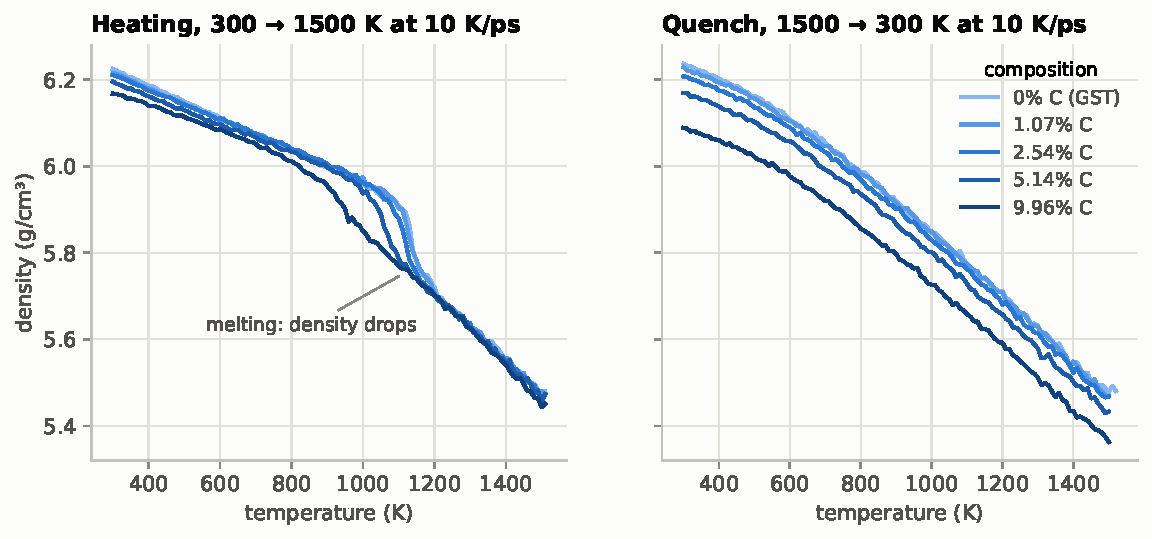
\includegraphics[width=\textwidth]{density_vs_T.pdf}
\caption{Density on the 10\,K/ps heating ramp (left; the drop near 1100\,K is melting of the superheated crystal)
and on the quench (right), mean of three replicas per composition.}
\label{fig:rhoT}
\end{figure}

\begin{figure}[htbp]
\centering
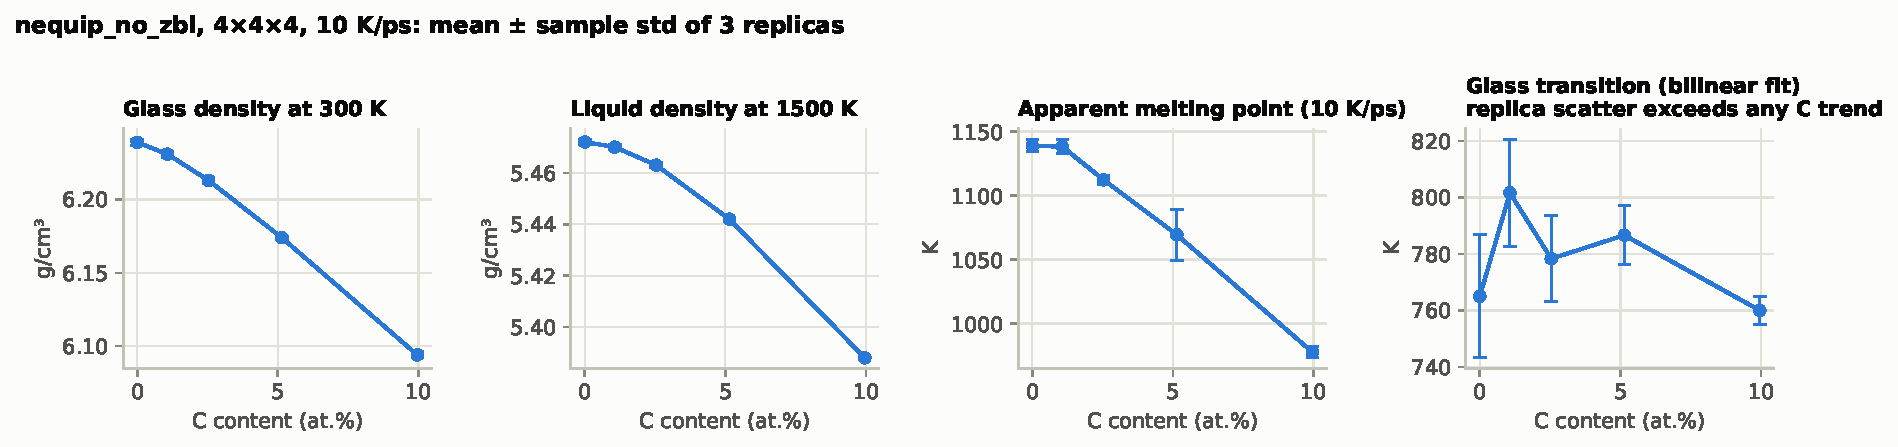
\includegraphics[width=\textwidth]{properties_vs_C.pdf}
\caption{Glass and liquid density, apparent melting point and glass transition against C content
(Table~\ref{tab:props}), mean $\pm$ sample standard deviation of three replicas.}
\label{fig:props}
\end{figure}

Density falls with C, by 1.5\% in the liquid and 2.3\% in the glass from 0 to 10\% C (Fig.~\ref{fig:props}),
steadily and with a replica spread of at most 0.002\,g/cm$^3$. The 0\% C glass, 6.239\,g/cm$^3$, is as dense as this
model's rocksalt crystal (6.224\,g/cm$^3$ at 300\,K); experimentally the glass is 6--7\% less dense. The
model's glass matches the DFT reference's own cold melt-quenched glass to 0.01\% in density, so this is a property of
the reference, not of the fit.

The apparent melting point, the temperature of fastest enthalpy rise on the 10\,K/ps heating ramp, is flat to 1\%
C, then falls to 978\,K at 10\% C. It is a superheating limit,
an upper bound on the model's melting point. The glass transition from a bilinear fit of $V(T)$ on the quench
scatters by 5--22\,K between replicas with no trend in C, so the effect of C on $T_g$ is not resolved. Crystal-like
order in the glass (\texttt{xfracGST} 0.12--0.14) falls slightly with C to 5\% C.

\section{Structure of the glass}

\begin{figure}[htbp]
\centering
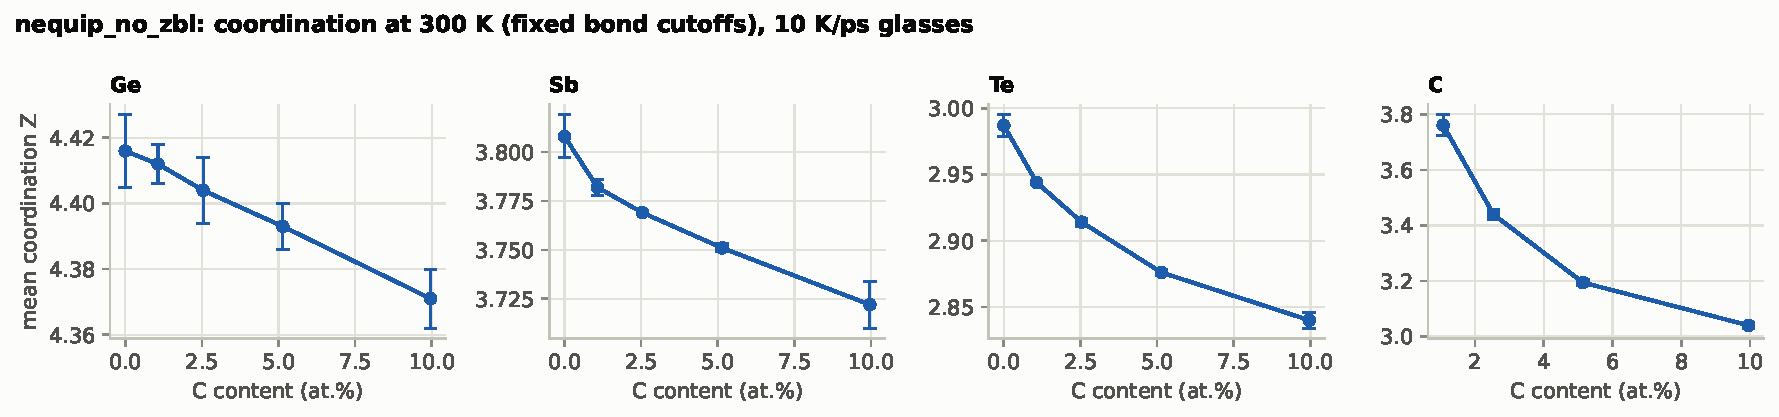
\includegraphics[width=\textwidth]{coordination_vs_C.pdf}
\caption{Mean coordination of each species at 300\,K against C content, mean $\pm$ sample standard deviation of three replicas.}
\label{fig:coord}
\end{figure}

\begin{figure}[htbp]
\centering
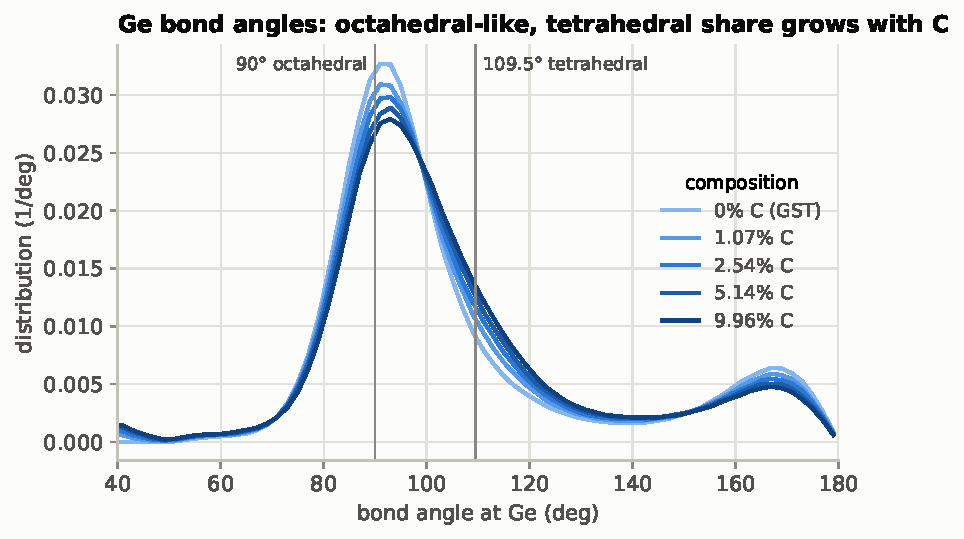
\includegraphics[width=0.49\textwidth]{ge_angles.pdf}\hfill
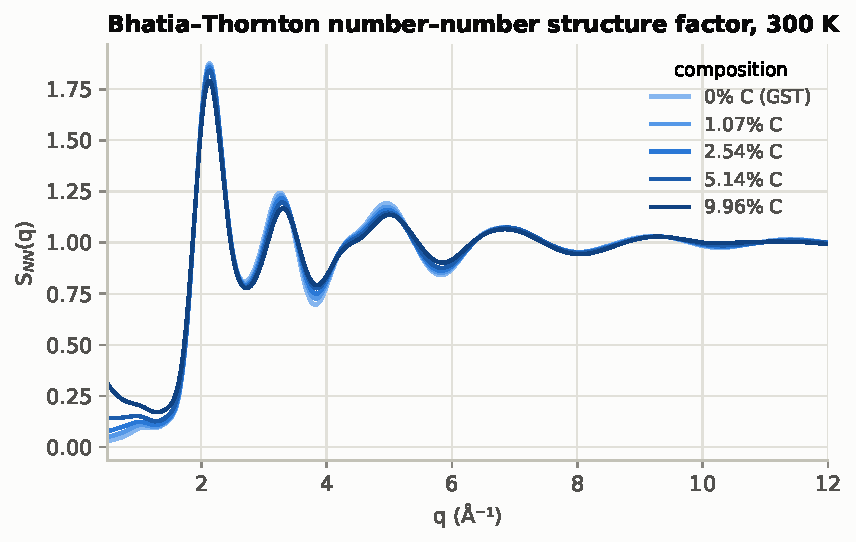
\includegraphics[width=0.49\textwidth]{sq_nn.pdf}
\caption{Left: bond-angle distribution at Ge. Right: Bhatia--Thornton number--number structure factor $S_{NN}(q)$.}
\label{fig:angles}
\end{figure}

Coordination drops slightly with C (Fig.~\ref{fig:coord}): Ge from 4.42 to 4.37, Sb from 3.81 to 3.72, Te from 2.99 to
2.84, a small, steady drop consistent with the lighter C-rich glass. C is 3.76-coordinated at 1\% C and 3.04 at
10\%. The Ge bond-angle distribution peaks at 91--93$^\circ$ (octahedral-like) for every composition, and the share
between 100 and 120$^\circ$ (tetrahedral-like) rises from 0.20 to 0.27 with C (Fig.~\ref{fig:angles}).

\section{Carbon clustering}

\begin{figure}[htbp]
\centering
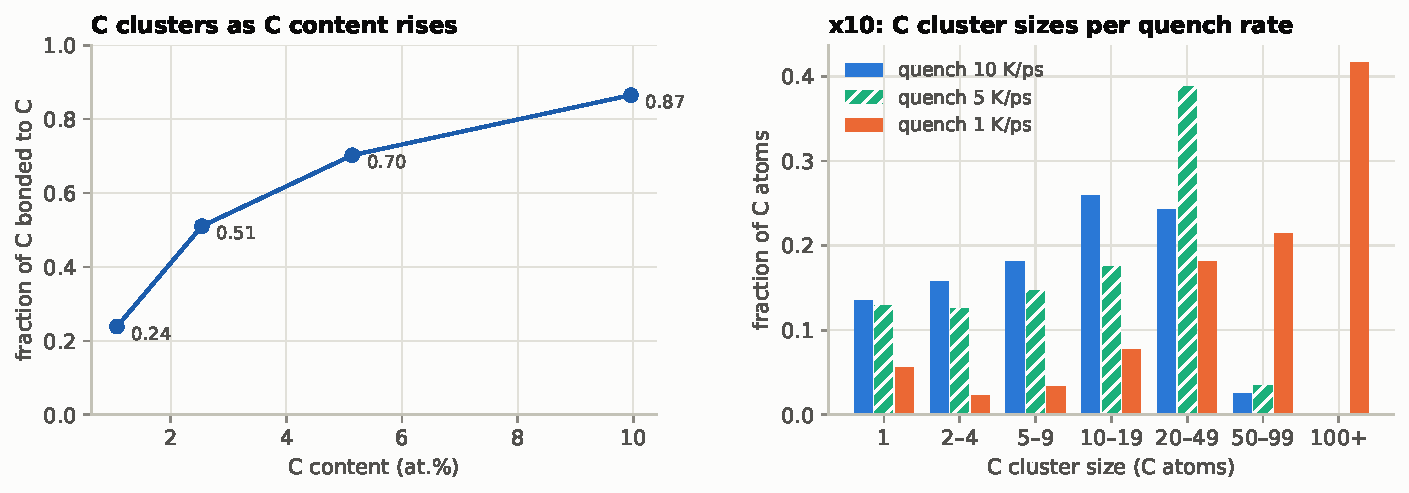
\includegraphics[width=\textwidth]{carbon_clustering.pdf}
\caption{Left: fraction of C atoms bonded to at least one other C. Right: C cluster sizes
in the 10\% C glass after each quench rate.}
\label{fig:cclust}
\end{figure}

\begin{figure}[htbp]
\centering
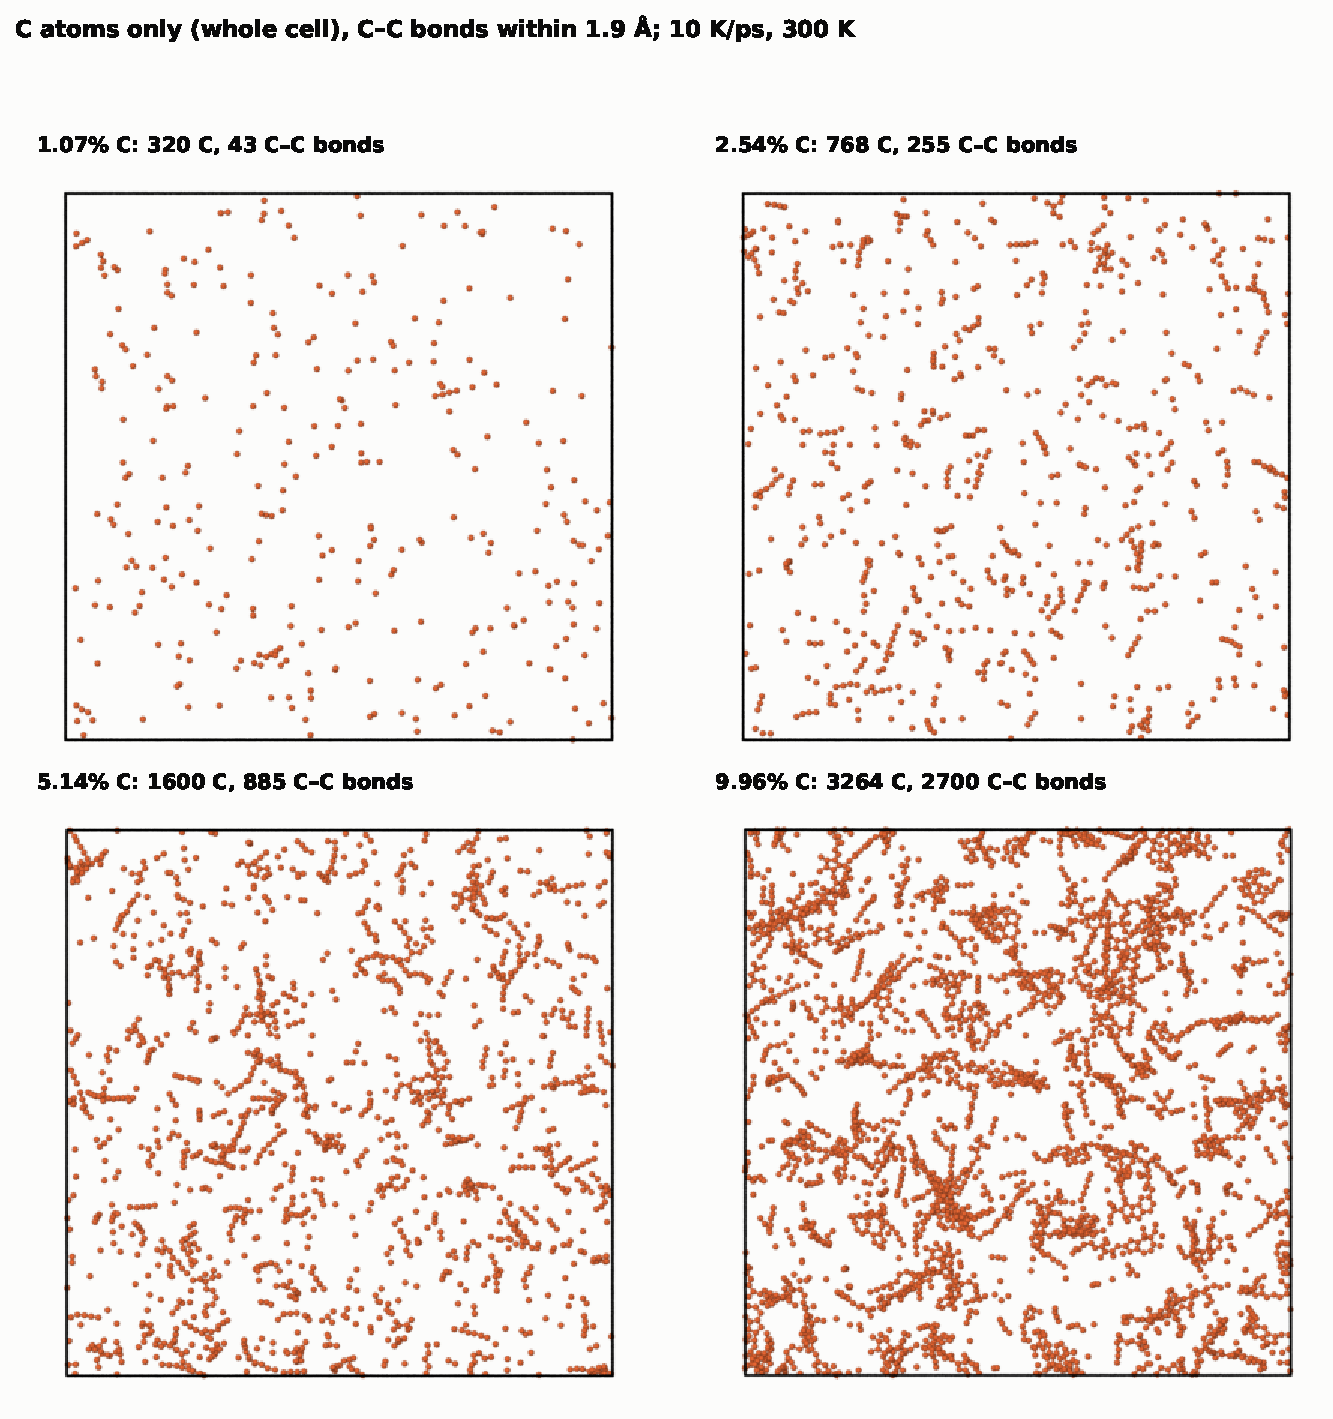
\includegraphics[width=0.78\textwidth]{render_c_network_all_grid.pdf}
\caption{C atoms only (whole cell seen along $z$) in the 10\,K/ps glasses at 300\,K, 1.07 to 9.96\% C; C--C bonds
within 1.9\,\AA. The projection makes some depth overlaps look like contacts.}
\label{fig:cnetall}
\end{figure}

\begin{figure}[htbp]
\centering
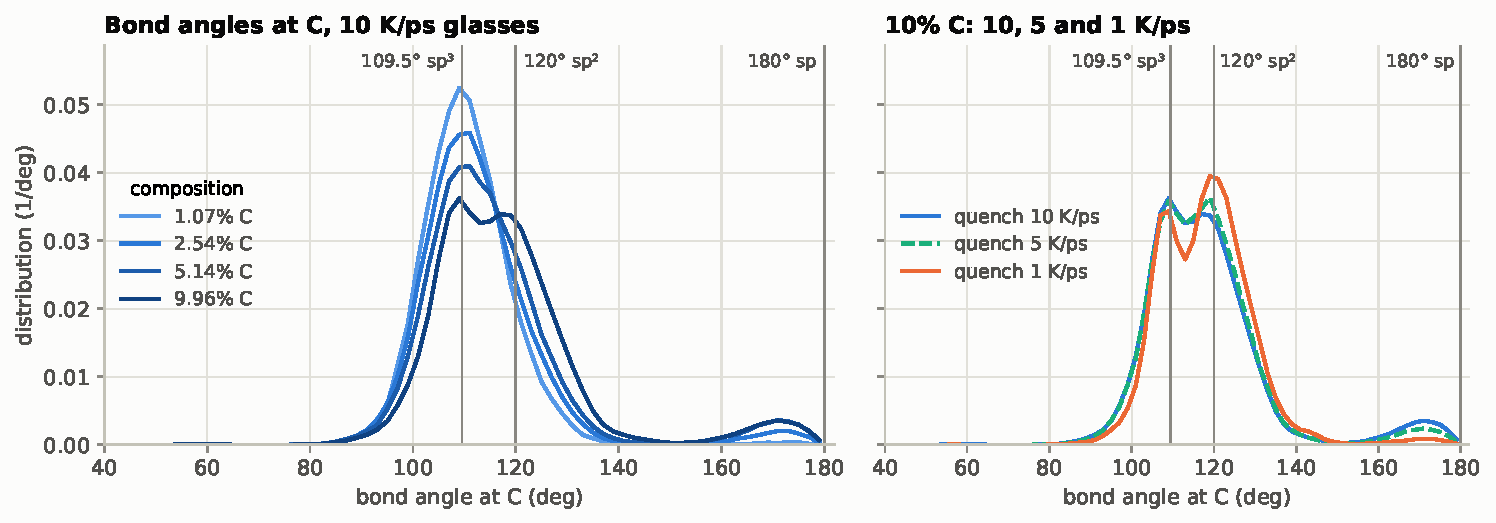
\includegraphics[width=\textwidth]{c_angles.pdf}
\caption{Bond-angle distribution at C. Left: 10\,K/ps glasses, 1.07 to 9.96\% C. Right: 10\% C after each quench
rate. Reference lines at the tetrahedral (sp$^3$), planar (sp$^2$) and linear (sp) angles.}
\label{fig:cang}
\end{figure}

C clusters at every content. The fraction of C atoms bonded to another C rises from 0.24 at 1\% C through 0.51 and
0.70 to 0.87 at 10\% C, with 0.26, 0.67, 1.09 and 1.63 C--C bonds per C atom (Figs.~\ref{fig:cclust},
\ref{fig:cnetall}). At 10\% C, 53\% of C sits in clusters of ten or more atoms, the largest of 69 atoms. The commonest C environments change from Ge/Sb-rich (Ge$_3$Sb 20\%, Ge$_2$Sb$_2$ 14\%,
Ge$_4$ 10\% at 1\% C) to C-rich (C$_2$ 17\%, C$_3$ 16\%, GeC$_2$ 14\% at 10\% C). C binds Ge before Sb before Te: at
10\% C there are 0.44 C neighbours per Ge atom, 0.18 per Sb and 0.04 per Te.

The C-centred bond angles (Fig.~\ref{fig:cang}) peak at 109$^\circ$ (sp$^3$-like) at 1\% C, with 61\% of angles
between 100 and 115$^\circ$. With more C the planar share grows: at 10\% C, 44\% of angles lie between 115 and
130$^\circ$ and 39\% between 100 and 115$^\circ$, a broad distribution between the two.

\section{Quench rate}
\label{sec:rate}

\begin{figure}[htbp]
\centering
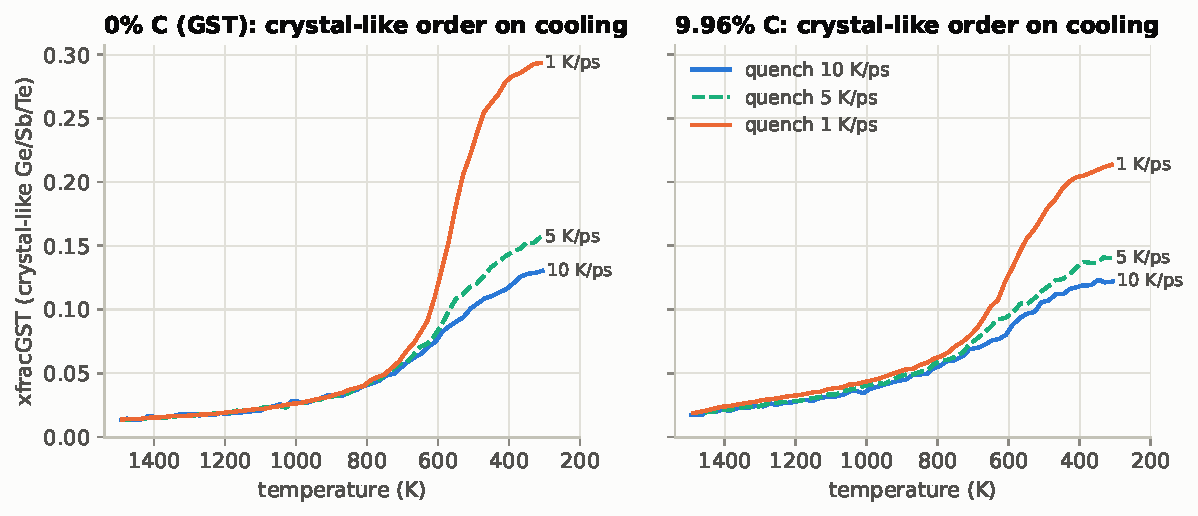
\includegraphics[width=\textwidth]{quench_order.pdf}
\caption{Crystal-like order of Ge/Sb/Te on cooling at 10, 5 and 1\,K/ps, for 0 and 10\% C (replica 1).}
\label{fig:rate}
\end{figure}

\begin{figure}[htbp]
\centering
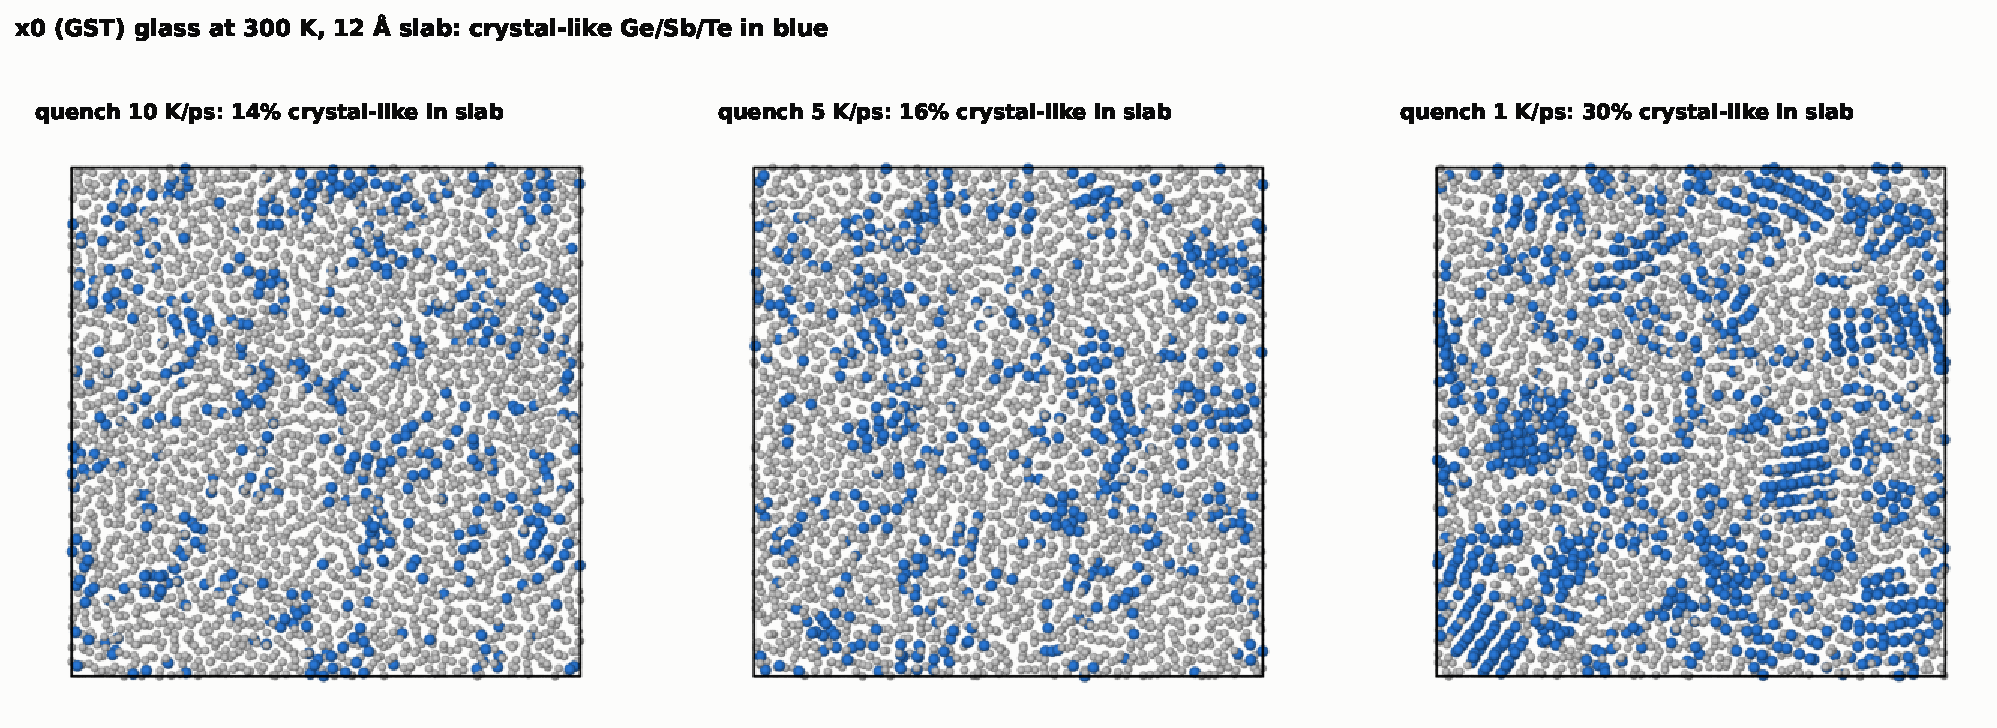
\includegraphics[width=\textwidth]{render_crystal_like.pdf}
\caption{The 0\% C glass at 300\,K after each quench rate, 12\,\AA{} slab: crystal-like Ge/Sb/Te atoms (in-run bond
count $\geq 4$) in blue.}
\label{fig:render}
\end{figure}

After a 1\,K/ps quench, \texttt{xfracGST} at 300\,K is 0.298 (0\% C) and 0.214 (10\% C), against
$0.142 \pm 0.008$ and $0.129 \pm 0.006$ after 10\,K/ps (Fig.~\ref{fig:rate}). It rises during the quench, mostly
between 650 and 450\,K for 0\% C and from 650\,K all the way down for 10\% C, and the 1\,K/ps slab shows ordered domains
with aligned atomic rows (Fig.~\ref{fig:render}): the glass partly crystallized on cooling. C slows this: the 10\% C glass ends lower. The 5\,K/ps glasses read 0.159 and 0.144, 0.015--0.017 above
the 10\,K/ps means (about two replica standard deviations, from one run each), with no ordered domains in the slab:
slightly more relaxed, not crystallized.

Density barely depends on rate: 6.239\,g/cm$^3$ at all three rates for 0\% C, and 6.094, 6.100 and 6.104\,g/cm$^3$
at 10, 5 and 1\,K/ps for 10\% C. At 1\,K/ps the coordination rises toward the octahedral crystal (0\% C: $Z_\text{Ge}$
4.52 against 4.42, $Z_\text{Te}$ 3.10 against 2.99) and the tetrahedral-like Ge share falls from 0.20 to 0.17. Slower
quenching also coarsens the C network (Figs.~\ref{fig:cclust} and \ref{fig:cang}): at 1\,K/ps, 94\% of C is bonded to C
and 89\% sits in clusters of ten or more atoms, up to 223 (10\,K/ps: 87\%, 53\%, 69), and the C bond angles turn
planar (peak 119$^\circ$, 51\% between 115 and 130$^\circ$). The recrystallization study therefore starts from the
10\,K/ps glasses.

\section{Bond-cutoff check}
\label{sec:cutoffs}

\begin{figure}[htbp]
\centering
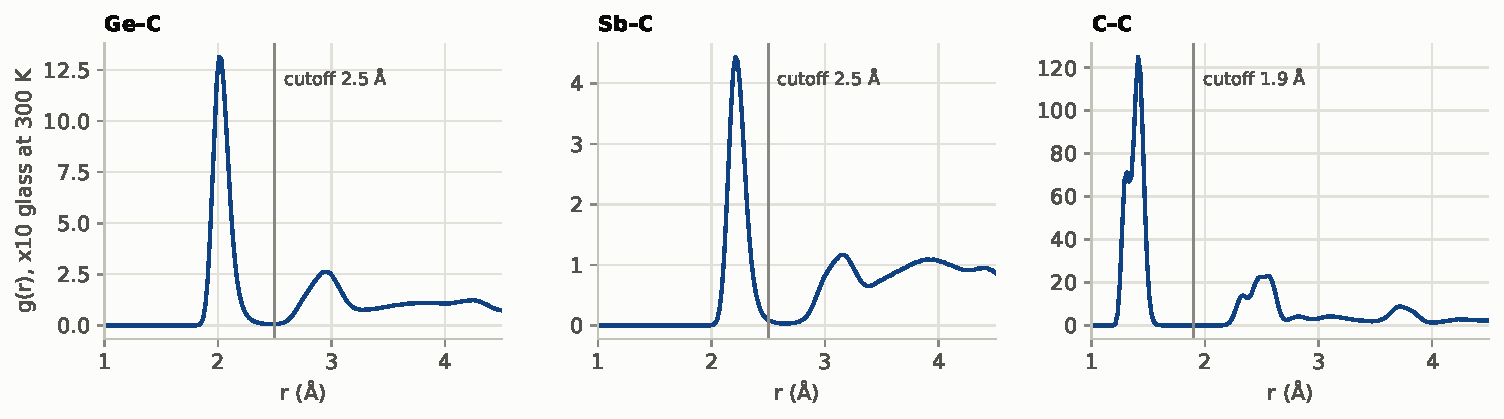
\includegraphics[width=\textwidth]{c_cutoffs.pdf}
\caption{Partial $g(r)$ for C pairs in the 10\% C glass (replica 1, 10\,K/ps) with the fixed bond cutoffs.}
\label{fig:cut}
\end{figure}

The C cutoffs were checked on this model's 10\% C glasses (Fig.~\ref{fig:cut}):
$g_\text{CC}(1.9\,\text{\AA}) = 0$ in all four (three at 10\,K/ps, one at 5\,K/ps). At 2.5\,\AA, $g$ is 0.05--0.07
for Ge--C and 0.09--0.11 for Sb--C, on the tails of peaks at 2.0 and 2.2\,\AA; moving the cutoff by $\pm0.1$\,\AA{}
changes the C coordination of Ge by under 1\% and of Sb by under 3\% (replica 1). The cutoffs were kept.

\section{Limitations}
\begin{itemize}
\item \textbf{Glass as dense as the crystal.} Experimentally the glass is 6--7\% less dense than the crystal; with
this model the two are equal. The DFT reference's own glass behaves the same
way, so conclusions that depend on the glass--crystal density difference belong to that reference.
\item \textbf{Rates.} Every quench rate here is many orders of magnitude faster than experiment; $T_{m,\text{app}}$
is a superheating limit and $T_g$ depends on rate.
\item \textbf{Single replicas at 5 and 1\,K/ps.} The rate comparison rests on one run per rate and composition,
against a replica spread of up to 0.008 in \texttt{xfracGST} at 10\,K/ps.
\item \textbf{One potential.} Every number here is \nozbl{}'s. Which conclusions depend on the potential, in
particular on the missing short-range term, will show when \texttt{nequip\_zbl} and \texttt{rushik\_zbl\_pairwise}
are run through the same protocol.
\item \textbf{Crystal-like order is not crystallinity.} Even the 10\,K/ps glasses hold crystal-like patches, a
baseline the recrystallization analysis accounts for.
\end{itemize}

\end{document}
